% !TEX encoding = UTF-8
\documentclass[fontsize=12pt,paper=letter,twoside]{scrartcl}
% Various imports and themes
\usepackage[top=4cm,bottom=4cm,left=3cm,right=3cm,asymmetric]{geometry}
%\geometry{landscape}
  % Activate for for rotated page geometry
%\usepackage[parfill]{parskip}    
  % Begin paragraphs with an empty line rather than an indent
\usepackage[table,xcdraw]{xcolor}
\usepackage{graphicx}

\usepackage{amsmath}
\usepackage{amssymb}
\usepackage{epstopdf}
\DeclareGraphicsRule{.tif}{png}{.png}{`convert #1 `dirname #1`/`basename #1 .tif`.png}
% Listings needs package courier
\usepackage{listings} % Needs 
\usepackage{courier}

\usepackage[framemethod=TikZ]{mdframed}
\usepackage{url}

\usepackage{sty/bsymb} %% Event-B symbols
\usepackage{sty/eventB} %% REQ and ENV
\usepackage{sty/calculation}
\usepackage{sty/mathpartir}

% \usepackage{sty/tikz-uml}


%Maths
\usepackage{amssymb,amsmath}
\def\Fl{\mathbb{F}}
\def\Rl{\mathbb{R}}
\def\Nl{\mathbb{N}}
\def\Bl{\mathbb{B}}
\def\St{\mathbb{S}}
\newcommand{\ovr}{\upharpoonright}
\newcommand{\var}[1]{\textit{#1}}
%Useful definitions
\newcommand{\mv}[1]{\textit{m\_#1}}
\newcommand{\cv}[1]{\textit{c\_#1}}
\newcommand{\degree}[1]{^{\circ}\mathrm{#1}}
%\newcommand{\comment}[1]{{\footnotesize \quad\texttt{--}\textrm{#1}}}
\newcommand{\im}[1]{i\texttt{-\!#1}}

\usepackage[headsepline]{scrpage2}
\pagestyle{scrheadings}
\ihead[]{\small EECS4312 Report1}
\ohead[]{\small \thepage}
\cfoot[]{}
\ofoot[]{}


%%%%PVS environment%%%%%%%%%%%%%%%%%%%
\lstnewenvironment{pvs}[1][]
    {\lstset{#1,captionpos=b,language=pvs,
    mathescape=true,
    basicstyle=\small\ttfamily,
    numbers=none,
    frame=single,
    % numberstyle=\tiny\color{gray},
    % backgroundcolor=\color{lightgray},
    firstnumber=auto
    }}
    {}
 %%%%%%%%%%%%%%%%%%%%%%%%%%%%%%%%
 
%%%%PVS environment%%%%%%%%%%%%%%%%%%%
\lstnewenvironment{events}[1][]
    {\lstset{#1,captionpos=b,language=events,
    mathescape=true,
    basicstyle=\small\ttfamily,
    numbers=none,
    frame=single,
    % numberstyle=\tiny\color{gray},
    % backgroundcolor=\color{lightgray},
    firstnumber=auto
    }}
    {}
 %%%%%%%%%%%%%%%%%%%%%%%%%%%%%%%%
 
%%%%Verbatim environment%%%%%%%%%%%%%%%%%%%
\lstnewenvironment{code}[1][]
    {\lstset{#1,captionpos=b,
    mathescape=true,
    basicstyle=\scriptsize\ttfamily,
    numbers=none,
    frame=single,
    comment=[l][\color{red}]{--},
    % keywords = [1]{"->"},
    % numberstyle=\tiny\color{gray},
    % backgroundcolor=\color{lightgray},
    firstnumber=auto
    }}
    {}

% \newenvironment{boxed}[1]
%    {\begin{center}
%    #1\\[1ex]
%    \begin{tabular}{|p{0.9\textwidth}|}
%    \hline\\
%    }
%    { 
%    \\\\\hline
%    \end{tabular} 
%    \end{center}
%    }
 %%%%%%%%%%%%%%%%%%%%%%%%%%%%%%%%
 
 %Text in a box
\newenvironment{textbox}
    {\begin{center}
    \begin{tabular}{|p{0.9\textwidth}|}
    \hline\\
    }
    { 
    \\\\\hline
    \end{tabular} 
    \end{center}
    }

\usepackage{hyperref}

%Highlight \hl{}
\usepackage{soul}

\usepackage{enumitem}
\newlist{mylist}{itemize}{1}
\setlist[mylist]{label=\textbullet,leftmargin=1cm,nosep}

\usepackage{multirow}

% Reduce space between figure and caption
%\usepackage{caption}
%\captionsetup[table]{font=small,skip=0pt}     %% Adjust here
%or equivalently 
\usepackage[font=small,skip=4pt]{caption}

% Indent equations
%\setlength{\mathindent}{1cm}

% Set the header

%\afterpage{\clearpage}
\usepackage{afterpage}
\usepackage{fancyvrb}

% Allow better table placement?
\renewcommand\floatpagefraction{.9}
\renewcommand\topfraction{.9}
\renewcommand\bottomfraction{.9}
\renewcommand\textfraction{.1}   
\setcounter{totalnumber}{50}
\setcounter{topnumber}{50}
\setcounter{bottomnumber}{50}
\usepackage{morefloats}
\usepackage[section]{placeins}

\newcommand{\pre}[1]{{#1}_{-1}}
\newtheorem{defn}{Definition}%[section]
\newtheorem{lemma}{Lemma}%[section]
\newtheorem{theorem}{Theorem}%[section]

%Sequents
\usepackage{bussproofs}

% Hide sections
\newif\ifhideproofs
%\hideproofstrue %uncomment to hide proofs

% Needed for TLA
% \input{tla/tla-style.tex} % style file for TLA
% Reduce space around equations
\setlength{\abovedisplayskip}{3pt}
\setlength{\belowdisplayskip}{3pt}


 
\usepackage{pdfpages}
%%%%%%%%%%%%%%%%%%%%%%%%%%%%%%%%%%%%%%%%%%%%%%%%%%%%%%%%%%%%%%%%%%%%%%%%%
\begin{document}
%%%%%%%%%%%%%%%%%%%%%%%%%%%%%%%%%%%%%%%%%%%%%%%%%%%%%%%%%%%%%%%%%%%%%%%%%
% Title and Authors
\newcommand{\mytitle}{
	EECS2311-W20 Project: Venn Create\\ User Manual
}
\ihead[]{\small \mytitle}
\title{\mytitle}
\author{
	Chidalu Agbakwa (216337784) \and
	Jihal Patel (216376436) 	\and
	Shangru Li (214488993) 		\and
	Robert Suwary (215446016)
}
% Display a given date or no date
\date{\today}
\maketitle
%%%%%%%%%%%%%%%%%%%%%%%%%%%%%%%%%%%%%%%%%%%%%%%%%%%%%%%%%%%%%%%%%%%%%%%%%
\subsection*{Revisions}
\begin{tabular}{|l|l|p{3in}|}
	\hline
	Date & Revision& Description \\ 
	\hline
	09 February 2020 
	& 1.0       
	& Initial release of this document\\ 
	\hline
\end{tabular}
\bigskip\bigskip
%%%%%%%%%%%%%%%%%%%%%%%%%%%%%%%%%%%%%%%%%%%%%%%%%%%%%%%%%%%%%%%%%%%%%%%%%
\newpage
\vspace*{2in}
\begin{center}
	\huge{\textbf{User Manual}:\\ Venn Create}
\end{center}
\newpage
%%%%%%%%%%%%%%%%%%%%%%%%%%%%%%%%%%%%%%%%%%%%%%%%%%%%%%%%%%%%%%%%%%%%%%%%%
\newpage
\tableofcontents
\newpage
\listoffigures
%\listoftables
%%%%%%%%%%%%%%%%%%%%%%%%%%%%%%%%%%%%%%%%%%%%%%%%%%%%%%%%%%%%%%%%%%%%%%%%%
\newpage
\section{Introduction}
Welcome to Venn Create - a desktop application that can draw customizable
Venn diagrams.

Venn Create enables user to easily create Venn diagrams with customized
labels, in different size and shape. Which can be used to compare and
contrast two or more objects, events, people, or concepts. Clearly
illustrating the differences and similarities between different entities
and all of this, with ZERO cost.

Venn Create provides a user-friendly interface, so that new users will
be able to use the application with minimum efforts. In addition,
the application provides essential functionalities, such as export/import
existing Venn diagrams, printing and customized theming.

%%%%%%%%%%%%%%%%%%%%%%%%%%%%%%%%%%%%%%%%%%%%%%%%%%%%%%%%%%%%%%%%%%%%%%%%%
\newpage
\section{Get Started}

Venn Create provides an intuitive interface and strive to deliver the best user experience.

\subsection{Introduction Interface}

 After user opens the application, the introduction interface will display:

\begin{figure}[hbt]
	\begin{mdframed}
		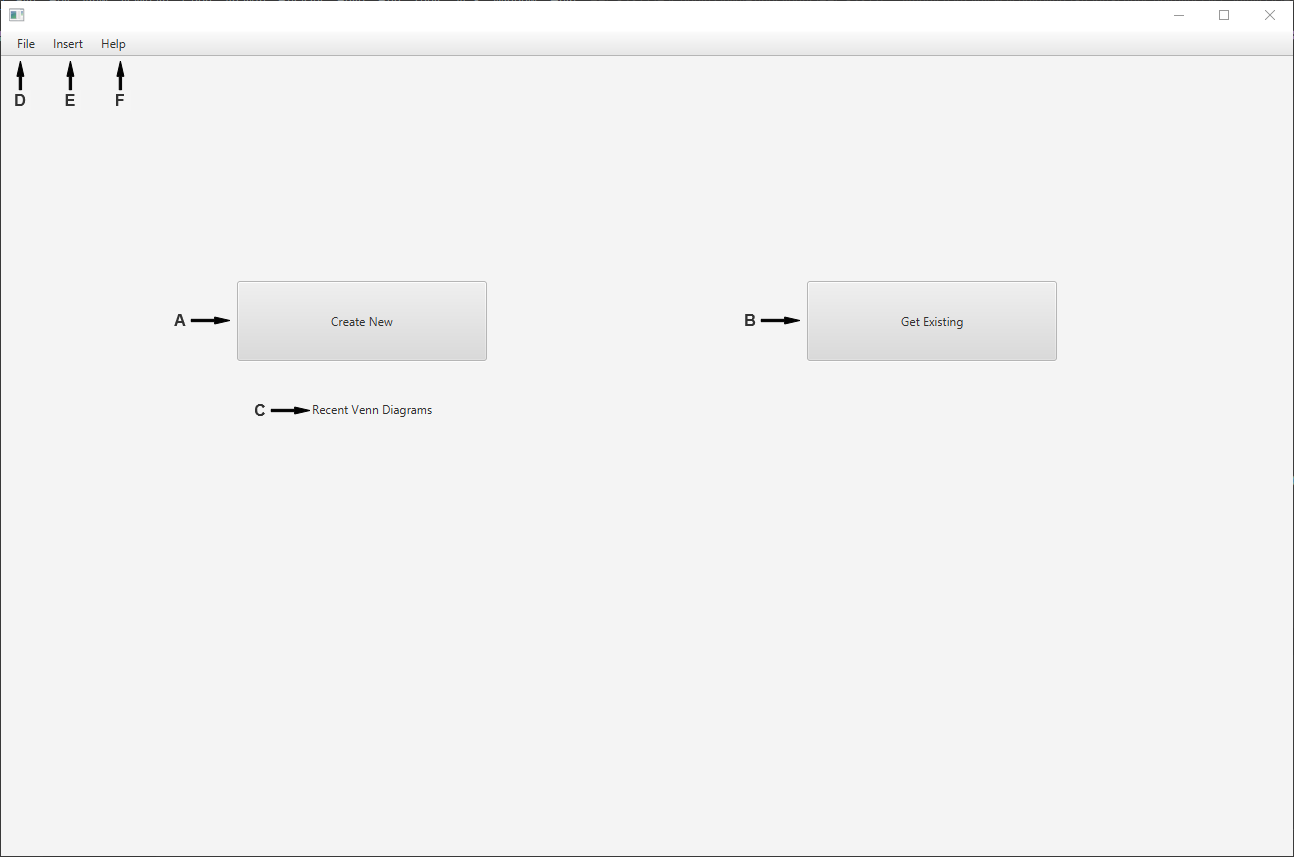
\includegraphics[width=\textwidth]{images/intro-screenshot.png}
	\end{mdframed}
	\caption{Introduction Interface}
\end{figure}

\begin{itemize}
	\item[\textbf{A.}] {
		Button to create a new Venn diagram.
	}
	\item[\textbf{B.}] {
		Button to import existing Venn diagrams.
	}
	\item[\textbf{C.}] {
		History list containing a record of the recent Venn diagrams.
	}
	\item[\textbf{D.}] {
		Menu bar button to expand the options for operations regarding files.
	}
	\item[\textbf{E.}] {
		Menu bar button to expand the options for inserting a new Venn diagram.
	}
	\item[\textbf{F.}] {
		Menu bar button to view the help page.
	}
\end{itemize}

\subsection{Main Interface}

If user chose to create or import any Venn diagrams, the application will switch to the main interface:

\begin{figure}[hbt]
	\begin{mdframed}
		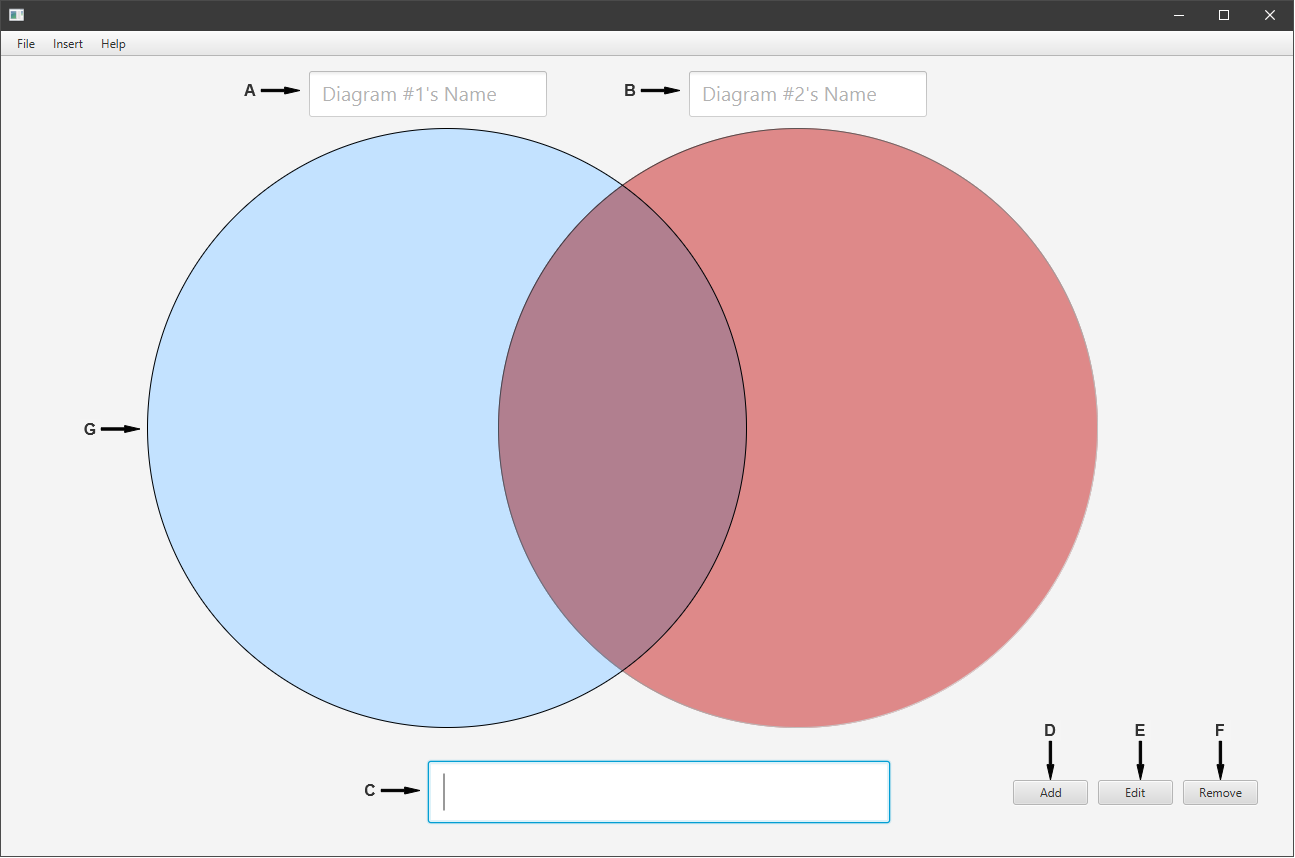
\includegraphics[width=\textwidth]{images/main-screenshot.png}
	\end{mdframed}
	\caption{Main Interface}
\end{figure}

\begin{itemize}
	\item[\textbf{A.}] {
		Text area for the name of the left Venn diagram.
	}
	\item[\textbf{B.}] {
		Text area for the name of the right Venn diagram.
	}
	\item[\textbf{C.}] {
		Text area for the content of the new text label to be added to the Venn diagrams.
	}
	\item[\textbf{D.}] {
		Button to add the a new text label to the Venn diagrams.
	}
	\item[\textbf{E.}] {
		Button to edit an existing text label of the Venn diagrams.
	}
	\item[\textbf{F.}] {
		Button to remove an existing text label from the Venn diagrams.
	}
\end{itemize}

%%%%%%%%%%%%%%%%%%%%%%%%%%%%%%%%%%%%%%%%%%%%%%%%%%%%%%%%%%%%%%%%%%%%%%%%%

\newpage
\section{Using the Software}

After getting acquainted with the basic user interface of the software.
User can explore the product and create customized Venn diagram. Here is an example usage:

\textbf{\begin{figure}[hbt]
		\begin{mdframed}
			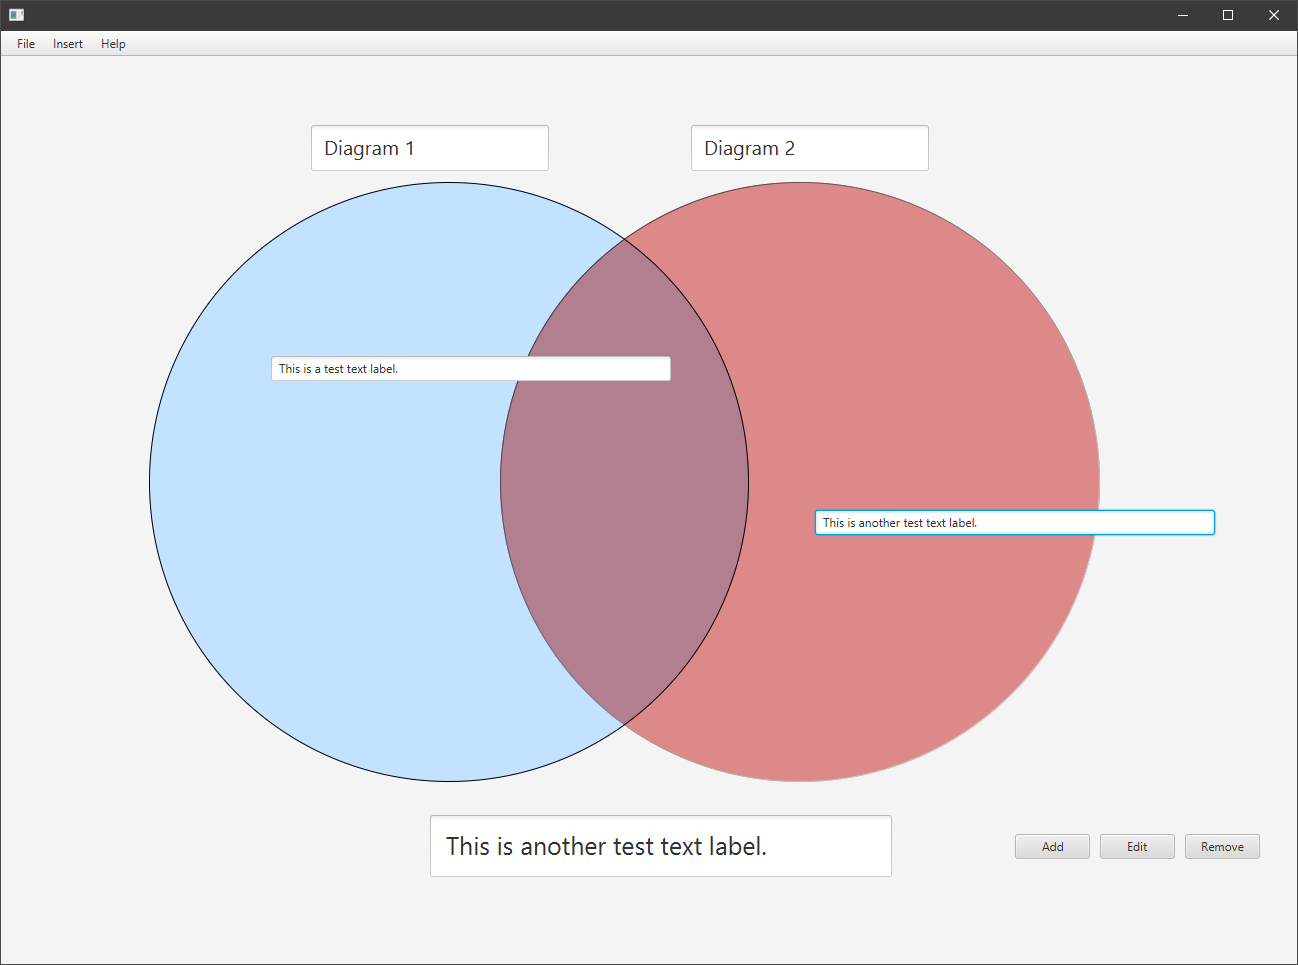
\includegraphics[width=\textwidth]{images/usage1-screenshot.png}
		\end{mdframed}
		\caption{Example Usage}
\end{figure}}

In this use case, user named the left diagram "Diagram 1" and the right diagram "Diagram 2".

Furthermore, user has already added two text label on the Venn diagrams. Note that, after each text label been added, user can drag it to anywhere on the workplace.

If user wish to add more text label, one can input the content of the new label and click `Add` button. Then drag the new label anywhere needed.

%%%%%%%%%%%%%%%%%%%%%%%%%%%%%%%%%%%%%%%%%%%%%%%%%%%%%%%%%%%%%%%%%
\end{document} 	

